% Final paper, CSE 216 / COGS 230, Fall 2026.
% Single-column ACM CHI format: acmart with the manuscript option.
% Compile with: sh build.sh (uses the ACM class in template/). Check with: python3 scripts/check_build.py
% Every number traces to the file named in the nearest "% src:" comment. Paths are relative to Final_Project/.
\documentclass[manuscript,screen]{acmart}

\usepackage{longtable}
\usepackage{graphicx}
\graphicspath{{figures/}}

\setcopyright{none}
\settopmatter{printacmref=false}
\renewcommand\footnotetextcopyrightpermission[1]{}
\acmConference[CSE 216 / COGS 230]{Final paper}{Fall 2026}{}
\acmYear{2026}
\acmDOI{}
\acmISBN{}

\newcommand{\code}[1]{\texttt{#1}}

\begin{document}

\title[Offloading or Surrendering?]{Offloading or Surrendering? Mapping Where AI Assistance Substitutes for Thinking in Formal Long-Form Writing}

% TODO(Wayne): replace the affiliation line with your institution, city and preferred email.
\author{Wayne Wang}
\affiliation{%
  \institution{CSE 216 / COGS 230, Fall 2026}\city{[city]}\country{USA}
}

\begin{abstract}
Generative AI now sits inside how people write, and research on it has divided over a basic question: when does handing work to a model support a writer's thinking, and when does it replace that thinking? Theories separate cognitive offloading from cognitive surrender, but they define surrender by missing deliberation, which no writing tool can observe. Tools see only logs. This paper asks which logged behaviors go with support and which with substitution, and which of those a tool could act on. The study analyzes existing logs from NIRVANA, a timed essay study with chat and editor records, and from WildChat, a corpus of in-the-wild conversations. No participants were recruited. AI agents coded 528 request windows, and a rule table frozen before new labels were read turned each window's codes into a category tied to published definitions. No human coded the data. Across 106 sessions (3 capped at ten turns), categories were assigned window by window. In the 71 NIRVANA sessions, the only ones with editor records, pasting did not separate the two sides. Whose content was pasted, and what the writer did next, did. Sessions with more unchecked adoption of AI text ended with more AI text in the essay and lower felt ownership. In NIRVANA, two content-free log events caught 63\% of the windows that the AI-coded labels mark as surrender-leaning. The contribution is a framework that links observable behavior to likely offloading or surrender, session-level findings, and log-only signals for in-situ feedback.
\end{abstract}

\begin{CCSXML}
<ccs2012>
   <concept>
       <concept_id>10003120.10003121.10011748</concept_id>
       <concept_desc>Human-centered computing~Empirical studies in HCI</concept_desc>
       <concept_significance>500</concept_significance>
   </concept>
 </ccs2012>
\end{CCSXML}
\ccsdesc[500]{Human-centered computing~Empirical studies in HCI}
\keywords{AI-assisted writing, cognitive offloading, cognitive surrender, log analysis, qualitative coding, in-situ feedback}

\maketitle

\section{Introduction}

Large language models are now ordinary writing tools, and the evidence on what they do to their users points in several directions. Unguarded GPT-4 raised high school students' practice performance, while students could underperform once it was taken away \cite{bastani2025}. Gains from AI access lasted for students who used it as a tutor and faded for those who had it write \cite{contractor2026}. Writers who use AI report lower psychological ownership of the result \cite{joshi2025}. These studies say that the outcome depends on how the tool is used. They do not say how a particular use looks while it is happening.

That gap matters because a writing tool can act only on what it can see. \citet{risko2016} define cognitive offloading neutrally, as physical action that reduces cognitive demand. \citet{shaw2026} separate strategic delegation, where a person's reasoning stays active, from cognitive surrender, the uncritical adoption of AI output. The second definition rests on absent deliberation, and no log records deliberation. Interfaces that want to intervene need a defensible way to go from behavior to concept.

This paper builds that link for formal long-form writing. It analyzes existing logs from NIRVANA, in which university students wrote a timed essay with ChatGPT while chat and editor events were recorded \cite{jelson2026nirvana}, and WildChat, a corpus of ChatGPT conversations collected in the wild \cite{zhao2024}. I recruited no participants. AI agents coded each request, the AI's response and the writer's next action on observable behavior only, and a frozen rule table mapped each window's codes to one category with a stated strength and a cited source. No human coded the data, and all reported agreement is between AI models. Section~\ref{sec:limitations} collects the constraints.

\begin{description}
  \item[RQ1 (Boundary).] Across the activities of formal long-form writing, which observable patterns of AI use are associated with supporting the writer's thinking (offloading), and which with substituting for it (surrender)?
  \item[RQ2 (Awareness).] Which of these substitutions are likely to be visible to the writer, and which are not?
  \item[RQ3 (Signals).] What observable features of human-AI writing interactions could indicate substitution and serve as a basis for in-situ feedback?
\end{description}

The findings are four theses. T1: pasting is not the line between support and substitution; whose content moves and what the writer does next are. T2: the writer's own text is the anchor. T3: surrender-leaning windows leave little work on the text. T4: in NIRVANA, two events that need no reading of content, a request on a near-empty page and a large paste with little typing, flag substitution risk.

\paragraph{Contributions.} This paper makes three contributions to HCI research on AI-assisted writing: (1) a framework that links observable behavior to likely offloading or surrender through the literature, as a five-question codebook and a frozen, source-cited rule table (Appendix~\ref{app:codebook}); (2) session-level findings on where the boundary falls, from joining the codes to timing, typing and essay outcomes; and (3) log-only signals for in-situ feedback, each paired with a proposed intervention, not built or tested.

Section~\ref{sec:related} reviews related work, Section~\ref{sec:method} gives the method and Section~\ref{sec:results} the results. Sections~\ref{sec:barriers} and~\ref{sec:limitations} report barriers and limitations, Section~\ref{sec:discussion} answers the research questions and Section~\ref{sec:conclusion} concludes. The appendices hold the codebook, the agreement table, the session archetypes and the AI use table.

\section{Related Work}
\label{sec:related}

Research on thinking with external tools treats offloading as a neutral act whose value depends on the goal \cite{risko2016}, and writing as planning, translating and reviewing under a monitor \cite{flower1981}, a frame recent work adapts to AI \cite{yukita2025,wan2024}. Generative AI has fractured the vocabulary: \citet{shaw2026} name surrender as uncritical adoption, PAUSE and Maier et al.\ use ``offloading'' for the harmful substitution itself \cite{alam2026,maier2026}, and others draw the line between dependent and autonomous offloading \cite{zhu2026} or along axes of cognitive labor and oversight \cite{kim2025arcp}. Consequences differ with the use. Unaided performance falls in some settings \cite{bastani2025} and depends on the form of help in others \cite{maier2026,contractor2026}, small or self-reported studies add weaker signals of reduced engagement \cite{kosmyna2025,lee2025}, and ownership moves separately from contribution \cite{joshi2025,park2026,jelson2026chi}. People may also misjudge AI's part in their work \cite{kim2026fallacy,skulmowski2024,tankelevitch2024,bhat2026}.

The closest studies read AI-assisted writing from traces. NIRVANA clusters 77 students into four profiles from contribution and revision ratios \cite{jelson2026nirvana}, and related work codes queries against writing processes \cite{jelson2026chi} or finds temporal patterns across a session \cite{yang2025}. Request-focused studies code what is asked: who directs the work and at what scope separates learners where volume of use does not \cite{poquet2026}, idea and reasoning offloading carry the largest negative associations with later unaided thinking \cite{chen2026}, and follow-up turns fall into a small set of behaviors \cite{mysore2025}. Reliance measures reduce traces to a number \cite{welzel2026,padmakumar2026,davalos2026}, including a Reliance Index whose author states that it describes behavior without establishing surrender \cite{mallissery2026}. Requiring written justification cuts adoption of planted flaws while the justifications stay superficial \cite{tao2026}, which shows why a stated reason is weak evidence, and design reviews organize how co-writing systems might respond \cite{reza2025}.

What is missing is one account that ties request, origin of content, visible check and uptake together in one interaction, carries it across whole sessions, and joins it to the log and the finished text. Poquet, Chen and Mysore each code part of this, NIRVANA measures uptake but not why it happened, and theory defines surrender by a state that logs cannot show, so an interface designer has no stated route from event to concept. This literature shaped the project in two ways: the offloading-versus-surrender pairing in RQ1 is treated as one stipulation among several, using Risko and Gilbert's sense of offloading with Shaw and Nave's condition that reasoning stays in charge, and fields already coded by others are credited rather than claimed. The response is deliberately narrow: an explicit, frozen, source-cited mapping from behavior to category, applied to whole sessions.

\section{Method}
\label{sec:method}

This is a secondary analysis of existing logs that combines qualitative coding, a rule-based inference step and quantitative analysis of sessions. The supplementary details file gives the full procedure.

\subsection{Data}
\label{sec:data}

\textbf{No participants were recruited for this study.} I gave no instructions to anyone, paid no one and collected no new data. RQ2 is analytic, because the project promised no user study.

\emph{NIRVANA} \cite{jelson2026nirvana} records 77 university students writing an analytical essay of about 30 minutes with ChatGPT, including keystrokes, full conversations and all text copied from ChatGPT. Six never asked ChatGPT anything, so the 347 request windows come from 71 students. Its participant sheet gives two outside outcomes for each essay: GPT Final \% (the share of the essay that came from the AI) and Perceived Ownership (1--7). The sections of the NIRVANA preprint read for this project left no record of its consent or compensation procedures, so I state none here.
% TODO(Wayne): open the NIRVANA preprint (arXiv:2604.07344) and add its recruitment, consent and compensation details if it states them. Nothing here was read for those details, and no download was made in this draft.
% TODO(Wayne): add an IRB determination sentence if you obtained one. None is recorded in the project files.
% src: data/REPORT.md; data/raw/nirvana (sheet columns only); analysis/derived/outcome_nirvana.csv

\emph{WildChat} \cite{zhao2024} comes from users of a free ChatGPT service who opted in to anonymous collection. That is the only consent and compensation information I report for it. It has no editor, no verified identity and no record of what happened to the text afterward. An LLM screened conversations for formal long-form writing under a definition committed before any record was labeled. The coded sample comes only from a random seed of 1,200 of the 139,736 eligible conversations (837,989 before filtering), one conversation per IP cluster: 35 whole conversations with 151 windows, plus 30 earlier windows that stay out of every session measure. The supplementary details file shows the full funnel. In all, 528 windows were coded, and 106 whole sessions were analyzed. Dataset text stays out of the public record, and narratives in this paper are paraphrases.

\subsection{Codebook and coding}

The unit of coding is the \emph{window}: one request, the AI's response, and the writer's first relevant next action before the next request. Codes describe behavior and never cognition, because a writer may read and judge silently. Each window is coded on five questions (Appendix~\ref{app:codebook}). Q1 records the operation requested, from which a script derives the writing stage. Q2 records what the writer asks for. Q3 records where the response's main content came from and what the next action shows: \code{D0} no substantive decision, \code{D1} the writer's content, \code{D2} an AI proposal left open, \code{D3} the writer chose or revised, \code{D4} the AI proposal taken. Q4 records only visible checks of this response, from \code{V0} (none) through \code{V4} (compared with a source). Q5 records uptake, from \code{U1} (pasted unchanged) through \code{U7} (the writer types new text) and \code{U8} (moved on). A \code{prior\_own\_work} field records whether the writer's own draft is visible before the request. Agents revised a codebook reconstructed from the proposal and Milestone 1 through four pilot rounds (132 windows), and version 1.1 was frozen on November 6, 2026.
% TODO(Wayne): confirm who wrote codebook v1.0 (it says it is a reconstruction dated Nov 2; the repo cannot show the author).

All windows were coded by AI agents in Claude Code. Coder A (Claude Opus 5.5) and Coder B (Claude Sonnet 5.5) were instructed not to read each other's labels, and a transcript audit found that none did. A fresh Opus 5.5 adjudicator ruled on disagreements without knowing which coder was which. A Claude Fable 5.1 agent coded a 20-window set that had been reserved for human coding, which is a third AI check and not human validation. Across the three main coding runs, Cohen's $\kappa$ between coders, also reported in prior prompt coding \cite{jelson2026chi,poquet2026}, is 0.80 to 0.94 on \code{decision}, 0.79 to 0.94 on \code{verification} and 0.85 to 0.92 on \code{uptake} (Table~\ref{tab:agreement}). The rules applied to each coder's labels separately give the same category on 89.2\% of 528 windows ($\kappa = 0.86$).

\subsection{From codes to a category}
\label{sec:rules}

Codebook v1.2 adds an ordered rule table, R00--R20 and R99, in which the first match wins, so every window gets exactly one category. Each rule states a source and its main alternative reading. Strength grades the link between behavior and source, from \emph{strong} to \emph{weak}. A category is a literature-grounded inference from behavior. It is not a probability, not a measurement of cognition and not a judgment of the person. The rules were written from the sources, reviewed against 100 calibration windows, then frozen and hashed, and a script checks that hash before every analysis run. They gave a category other than indeterminate to 336 of the 428 windows outside calibration (78.5\%).

The surrender-leaning rules draw on uncritical adoption \cite{shaw2026}, copied answers \cite{bastani2025} and automation \cite{contractor2026}. The offloading rules draw on demand reduction \cite{risko2016} and on reasoning that stays active \cite{shaw2026}. The augmenting rules draw on augmentation \cite{contractor2026} and instrumental help \cite{maier2026}. Neutral-mechanical is a project category with no source. Two kinds of surrender-leaning window are kept apart. \emph{Request-only} windows come from R16: generation was requested and the output was iterated or left in chat, so no adoption is seen. \emph{Behavior-based} windows come from any other surrender rule, such as an unchecked paste. Offloading and augmenting together are called \emph{support}. Figure~\ref{fig:worked} walks two real windows through these steps, and Figure~\ref{fig:concept} places the categories on the dimensions that separate them.

\begin{figure}[tbp]
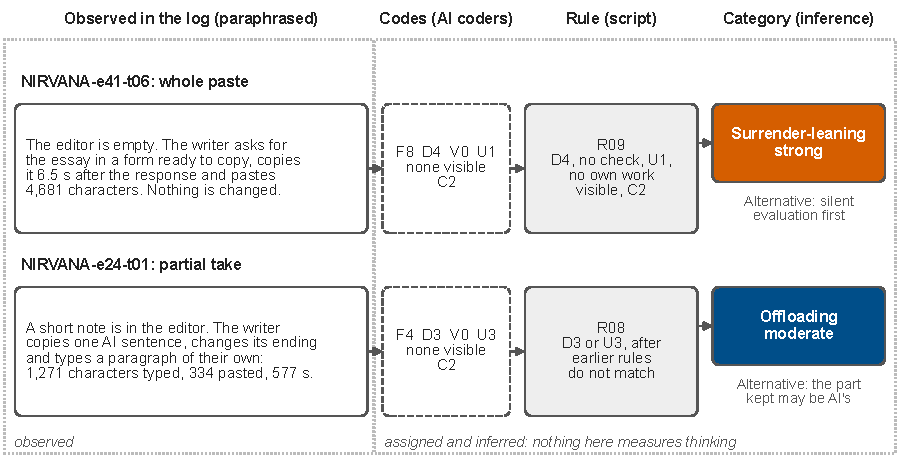
\includegraphics[width=\linewidth]{worked.pdf}
\caption{From behavior to inference, for a contrast pair of real windows (paraphrased; no dataset text). A whole paste (\code{D4}) and a partial take (\code{D3}) both move AI text into the editor. The codes record what happened, a frozen rule assigns the category, and the category stays an inference with a stated alternative reading.}
\Description{Two rows, each running left to right through four columns: observed in the log, codes, rule, and category. Row one, window NIRVANA-e41-t06: codes F8, D4, V0, U1, rule R09, category surrender-leaning, strong, alternative reading of silent evaluation first. Row two, window NIRVANA-e24-t01: codes F4, D3, V0, U3, rule R08, category offloading, moderate, alternative reading that the part kept may be AI's. A dotted boundary separates the observed column from the assigned and inferred columns.}
\label{fig:worked}
\end{figure}
% src: report/narratives.md s4, s5; inference/CSE216_Writing_Codebook_v1.2.md s9.3

\begin{figure}[tbp]
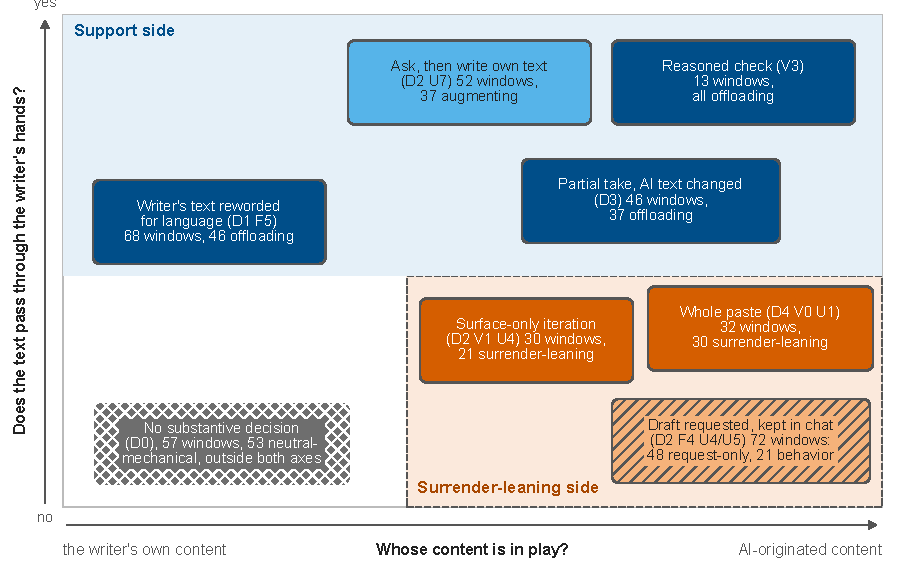
\includegraphics[width=\linewidth]{concept_map.pdf}
\caption{Concept map of the categories, with behavior signatures placed by hand on the two dimensions that separate them. Positions are schematic. Counts are windows in the 106 whole sessions, and the fill shows the most common category for that signature. Diagonal hatching marks the signature that is mostly request-only surrender-leaning, and cross-hatching marks neutral-mechanical, as in Figure~\ref{fig:archetypes}. A window can match more than one signature: 22 windows are in both surface-only iteration and draft requested. Indeterminate windows have no position on these axes.}
\Description{A two-dimensional map. The horizontal axis runs from the writer's own content to AI-originated content. The vertical axis asks whether the text passes through the writer's hands. Upper areas are the support side: writer's text reworded for language, ask then write own text, reasoned check, and partial take with AI text changed. The lower right is the surrender-leaning side: surface-only iteration, whole paste, and a draft requested and kept in chat, which is hatched and holds 48 request-only and 21 behavior-based windows. Neutral-mechanical sits in an unshaded corner, outside both axes.}
\label{fig:concept}
\end{figure}
% src: analysis/results/patterns.md s1; analysis/results/out_of_sample.md s3 (R02)

\subsection{Analysis}

From the raw NIRVANA logs a script extracted numbers only: for each window, the time from response to first copy and to next request (\emph{dwell}), the characters typed and pasted, and the editor's length at the request. WildChat stamps only AI turns. Categories were fixed before the new labels were read, and session types were then derived from the data by clustering category sequences. Order claims are tested against a within-session shuffle, outcome links are Spearman correlations with permutation $p$ values across sessions, and a logistic regression with session-cluster bootstraps tests the next-window prediction (procedure in the supplementary details file). Agents worked in Claude Code, and analysis scripts are Python with NumPy and Matplotlib. Data preparation, coding and analysis ran on November 6--7, 2026, and this draft was written on November 8. Every number reruns from saved labels by script.
% TODO(Wayne): standard citations for Cohen's kappa, Spearman, optimal matching and silhouette are not in lit/. This draft was limited to sources in lit/, so none is cited. Approve adding them or leave as is; see TODO_WAYNE.md.

\section{Results}
\label{sec:results}

The analysis method is in Section~\ref{sec:method}. Reasoned checks are nearly absent everywhere: of 498 whole-session windows, 376 show no check, 13 carry a reasoned challenge (\code{V3}) and none compare with a source (\code{V4}). In WildChat nothing shows what happened to the text, so 67 of its 69 surrender-leaning windows rest on the request alone.

The rule categories are the deductive themes (Section~\ref{sec:rules}). The inductive themes are six archetypes from clustering all 106 sessions, defined in Figure~\ref{fig:archetypes}: short support visit (35 sessions), long working session (21), paste into the draft (12), one-shot paste (7), delegate in chat (11) and unresolved (20). The two paste archetypes occur only in NIRVANA and end with essays almost wholly by the AI. Delegate in chat is mostly a WildChat pattern. Short support visits and long working sessions end with little AI text. The extremes show what the labels mean. In session e41 the editor stays empty while the writer asks for an essay and then only for longer or differently divided versions, and one paste of 4,681 characters follows. The essay is 100\% AI text by NIRVANA's measure, and the writer rated ownership 3.1 of 7. In session e24, after the first request, each request comes while a paragraph of the writer's is half written, and the writer answers each reply by typing a paragraph of their own. That essay is about 10\% AI text, with ownership 6.0.
% src: analysis/results/mining.md s1, s8, s10; analysis/results/out_of_sample.md s3, s7c; report/narratives.md s4, s5 (paraphrased)

\subsection{T1: the boundary is whether AI text passes through the writer's hands}

Pasting is on both sides. In NIRVANA, writers paste in 65.5\% of offloading windows and 63.8\% of behavior-based surrender windows. Figure~\ref{fig:after} shows what separates them: whose content was pasted and what followed. After taking most of an AI proposal, the writer types almost nothing and is back in the chat in about a minute. After taking part of one, the writer keeps typing for minutes.

\begin{figure}[tbp]
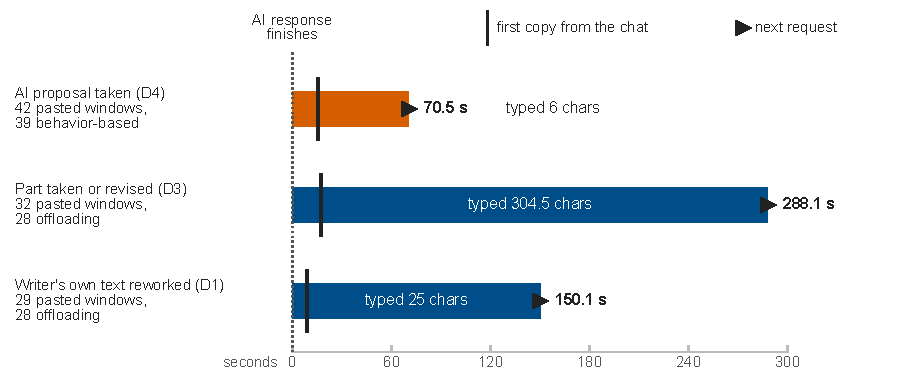
\includegraphics[width=\linewidth]{after_response.pdf}
\caption{What happens after the response, among NIRVANA windows with a paste, drawn to scale from medians. The bar runs from the end of the AI response to the next request (dwell), and the label gives the median characters typed. Dwell uses the 21, 23 and 20 windows that have a next request; typed medians use all pasted windows in each row. First-copy times come from the matching code signatures, not only pasted windows (\code{D4} with \code{U1}, 35 windows with a first copy; \code{D3}, 35; \code{D1}, 36).}
\Description{Three horizontal timelines to scale. AI proposal taken (D4), 42 windows, 39 behavior-based: dwell 70.5 seconds, 6 characters typed. Part taken or revised (D3), 32 windows, 28 offloading: dwell 288.1 seconds, 304.5 characters typed. Writer's own text reworked (D1), 29 windows, 28 offloading: dwell 150.1 seconds, 25 characters typed. A tick marks first copy at about 15, 17 and 9 seconds.}
\label{fig:after}
\end{figure}
% src: analysis/results/mining.md s5 "windows with any paste", s7 signature table

The finished essays show the same line. Across the 71 NIRVANA sessions, the share of behavior-based surrender windows tracks the share of AI text in the essay ($\rho = 0.60$, $p < 0.001$) and lower felt ownership ($\rho = -0.55$, $p < 0.001$). Request-only surrender tracks the AI share only weakly ($\rho = 0.19$, $p = 0.12$). Sessions with any behavior-based surrender window end with a median essay 81\% AI, and sessions without one end at 0\% (34 against 37 sessions). Pooled across datasets, requests that are not for generated prose are rarely surrender-leaning at any stage (7.1\% when planning, 9.8\% when reviewing), so substitution sits with requests for generated prose and what happens to them.
% src: analysis/results/mining.md s4, s8, s10

\subsection{T2: the writer's own text is the anchor}

Across NIRVANA sessions, the more text in the editor at the first request, the larger the session's support share ($\rho = 0.40$, $p < 0.001$, 65 sessions; on multi-window sessions alone 0.26, $p = 0.075$). Sessions whose first window shows a running draft have a mean support share of 0.77, against 0.71 with notes and 0.50 with nothing visible (Figure~\ref{fig:ownwork}). In WildChat, none of the 7 conversations that open with the writer's draft has a surrender-leaning window, and 18 of the 19 with no own work visible do.

The anchor also predicts the next step. A visible draft predicts lower odds that the next substantive window is surrender-leaning (odds ratio 0.23, 95\% session bootstrap 0.07 to 0.44), controlling for the current window's category, chat uptake, dataset and position. The rate, pooled across datasets, is 0.21 with a draft and 0.65 without, and most of this is between sessions: in the 16 sessions where the draft flag varies, it is 0.18 and 0.26. Sessions that become surrender-leaning return to support in 17 of the 29 NIRVANA sessions with a later window and 2 of 21 in WildChat.
% src: analysis/results/mining.md s3, s5, s6, s10

\begin{figure}[tbp]
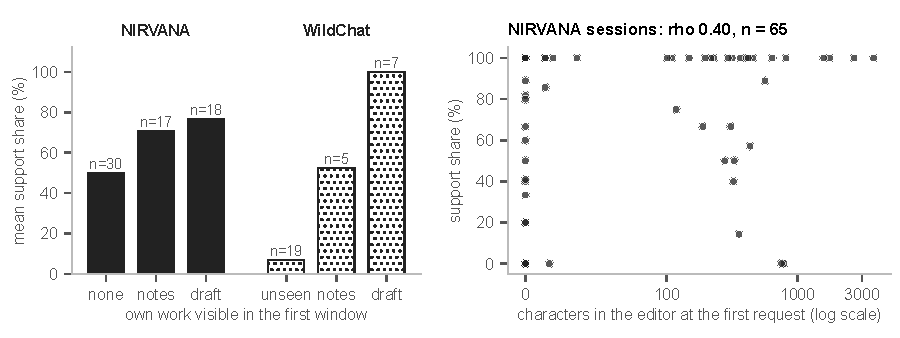
\includegraphics[width=\linewidth]{own_work.pdf}
\caption{Own work in the first window and the session's support share, by dataset (left), and NIRVANA editor length at the first request against support share (right). Support share is offloading and augmenting windows as a share of a session's windows with a surrender or support category; sessions with none, and one WildChat session whose first-window field is unsettled, are not shown. Unseen means a chat-only first window with no writer text.}
\Description{Left: bars of support share by first-window own work. NIRVANA none 50, notes 71, draft 77 percent. WildChat unseen 7, notes 53, draft 100 percent. Right: scatter of characters in the editor at the first request, on a log scale, against support share, with Spearman 0.401.}
\label{fig:ownwork}
\end{figure}
% src: analysis/results/mining.json own_work; analysis/derived/timing_nirvana.csv

\subsection{T3: surrender-leaning windows leave little work on the text}

In NIRVANA, the writer is back in the chat after a median of 57.8 seconds in surrender-leaning windows and 152.2 seconds in support windows (within-session shuffle $p < 0.001$). The gap is typing time (Figure~\ref{fig:dwell}). With under 50 characters typed, behavior-based surrender and support windows have the same dwell, 44.1 and 43.5 seconds. Median characters typed after the response are 0 for behavior-based surrender, 108 for offloading and 256 for augmenting. The copy is not faster: the first copy comes after a median of 15.5 seconds for behavior-based surrender and 10.35 seconds for support ($p = 0.62$). WildChat's only clock does not separate the sides (232 against 332 seconds, $p = 0.39$).
% src: analysis/results/mining.md s5, s7, s10

\begin{figure}[tbp]
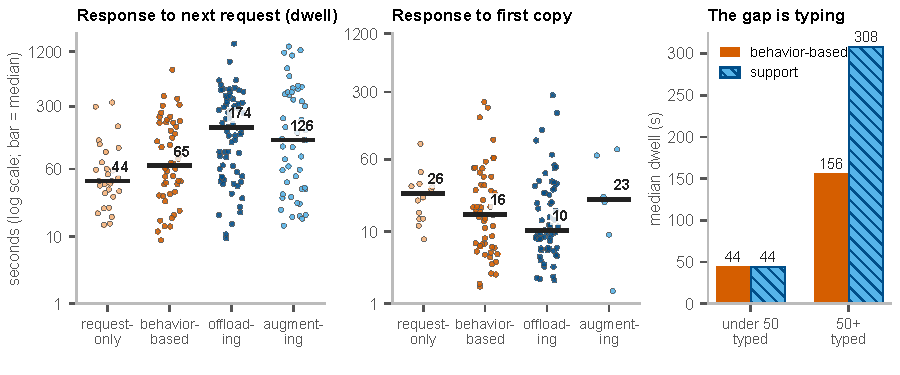
\includegraphics[width=\linewidth]{dwell.pdf}
\caption{NIRVANA dwell (left), time to first copy (center) and dwell split by how much was typed (right). Surrender-leaning windows end sooner, the copy is no faster, and with little typing the two sides have the same dwell. Dots are windows and bars are medians, in seconds. Support combines offloading and augmenting.}
\Description{Three panels. Left and center are strip plots on a log scale of seconds. Dwell medians: request-only 44, behavior-based 65, offloading 174, augmenting 126 seconds. First copy medians: request-only 26, behavior-based 16, offloading 10, augmenting 23 seconds. Right, a bar chart of median dwell: under 50 characters typed, behavior-based 44 and support 44 seconds; 50 or more typed, 156 and 308 seconds.}
\label{fig:dwell}
\end{figure}
% src: analysis/derived/timing_nirvana.csv; analysis/results/mining.md s7, s10

\subsection{T4: two content-free log events catch two-thirds of surrender-leaning windows}

Four rules were computed from the NIRVANA keystroke log alone, with no codes and no text, of which two are proposed as triggers (Figure~\ref{fig:triggers}). Together they fire on 140 of 347 windows, with precision 55.9\% against a base rate of 39.5\%, and catch 63.3\% of the windows that the AI-coded labels mark as surrender-leaning and 69.6\% of behavior-based ones. A large paste with little typing is the more precise of the two, and a request on a near-empty page catches more. Speed alone does not qualify: a quick return to the chat has only modest precision and no relation to essay outcome.
% src: analysis/results/mining.md s9, s10

\begin{figure}[tbp]
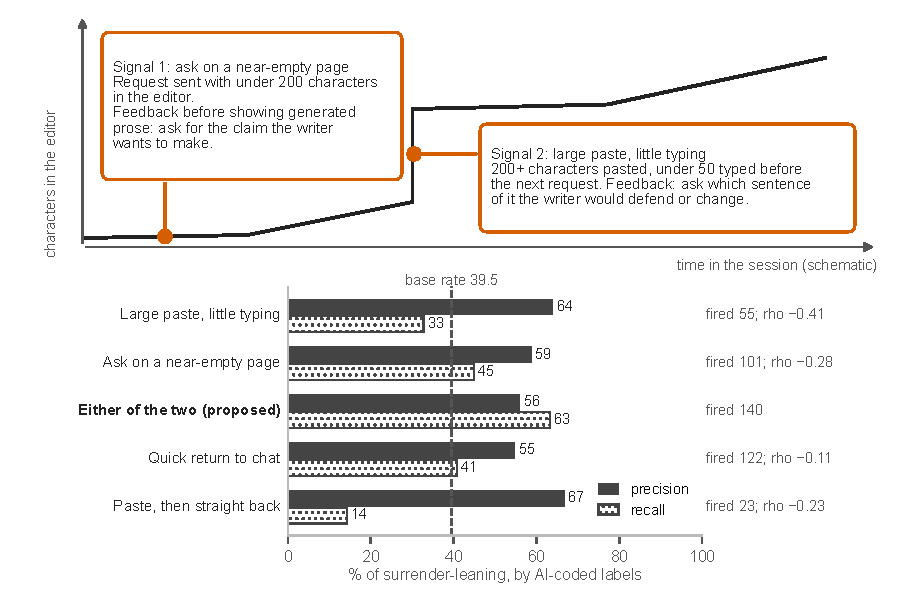
\includegraphics[width=\linewidth]{signals.pdf}
\caption{Top: where the two proposed log signals fire in a writing session, and the feedback each would give (schematic, not an interface; nothing was built). Bottom: performance of the log-only rules in NIRVANA, out of 347 windows. Precision is the share of fired windows with a surrender or support category that are surrender-leaning, against a base rate of 39.5\% on the same windows (98 of 248); recall is the share of all surrender-leaning windows caught, both by the AI-coded labels. Quick return: next request within 60 s of the response, with under 50 characters typed. Paste, then straight back: 200 or more characters pasted and the next request within 90 s. Rho is the correlation between a session's fire rate and felt ownership.}
\Description{Top: a schematic line of editor length over a session, with signal 1 near the start, when a request is sent with under 200 characters in the editor, and signal 2 at a sudden jump, when 200 or more characters are pasted and under 50 typed before the next request. Each has a feedback prompt. Bottom: paired bars of precision and recall against a base rate of 39.5 percent. Large paste, little typing: 64 and 33, fired 55. Ask on a near-empty page: 59 and 45, fired 101. Either of the two: 56 and 63, fired 140. Quick return to chat: 55 and 41, fired 122. Paste, then straight back: 67 and 14, fired 23.}
\label{fig:triggers}
\end{figure}
% src: analysis/results/mining.md s9, s10

\section{Analysis and Study Barriers}
\label{sec:barriers}
% TODO(Wayne): an agent drafted this section from the project logs, including every "What I learned" sentence. Rewrite any lesson that is not yours.

This section reports what did not go as planned in the process. Effects on the claims are in Section~\ref{sec:limitations}, and the supplementary details file has the full record.

\paragraph{The promise to be the primary coder was reversed.} My proposal said ``I remain the primary coder.'' On November 6 I chose agent-led work and kept a blind human coding set of 20 windows. Its instructions estimated 90 minutes to 2 hours and said the task could not be delegated. I delegated it anyway, to a Fable 5.1 agent. With more time, I would code those windows myself before seeing any AI output. \emph{What I learned:} the one step that later steps could not replace was the one I gave up.

\paragraph{The research-writing sample could not be reproduced.} Milestone 1 reported 42 clear candidates, below the target of 100 and unverified. A rebuild could not reproduce the count, and of 41 clear conversations on the rebuilt draw, 21 were not in English. On November 7 I widened the scope to formal long-form writing, under a definition committed before any record was labeled. \emph{What I learned:} a construct has to be defined and tested for precision before its count is reported.

\paragraph{Agents and tools broke assumptions.} Parallel sessions sharing a git index swept 27 files into one commit. Some agents broke the turn-by-turn reading protocol, which transcript audits caught. Automated access to several sources was refused, so a working-paper version of one paper was read. Review agents also caught real errors: a skeptic refuted 3 of 13 first-pass findings. \emph{What I learned:} a rule enforced only by instruction will sometimes be broken, so the audit has to be planned along with the rule.

\paragraph{What this taught me about doing research.} Most recoveries were possible because a decision had been written down before the data that would test it, and the failures came where something had been left implicit. With more time I would do less that scales and more that a person can check: code the 20 windows myself, test a screen's precision by hand before scaling it, and read the versions of record.

\section{Limitations}
\label{sec:limitations}

\paragraph{No human coded anything.} Every label comes from a model, and all agreement is AI-to-AI. Two models can share a bias, and shared rules can produce high agreement without correct labels. Adjudicators also leaned toward Opus Coder A, although category totals barely move (177 surrender-leaning windows in whole sessions under A's labels, 167 under B's and 167 in the final set).

\paragraph{Categories are inferences, and some links are built in.} A category says which pattern in the sources a window's behavior resembles. It does not measure thinking, and a writer may have evaluated AI text silently before pasting it. AI correctness is not coded. The categories in Figure~\ref{fig:after} restate the rules, and ``typed after'' partly restates how \code{D3} and \code{D4} are defined. The stage result is close to definitional, since drafting windows are generation requests. GPT Final \% measures AI text surviving in the essay, so its link to pasting is expected. Trigger precision and recall are partly built in, since pastes and an empty editor feed the codes they are scored against. They show that the events match the labels, not that they find surrender independently. Dwell and felt ownership are not built in, though dwell adds no signal beyond typing.

\paragraph{Evidence is uneven and correlational.} T3, T4 and the paste evidence for T1 rest on NIRVANA alone. In WildChat, surrender-leaning mostly means that someone asked for text, so cross-dataset contrasts mix behavior with what each log can see, and the gap in returning to support is a dataset difference, not an editor effect. The own-work and ownership links hold across sessions more than within them, so ``predicts'' means across sessions, and none of these results is causal. Tests are not corrected for multiple comparisons, so the theses rest on the large effects.

\paragraph{Sample and procedure.} NIRVANA is one timed essay by university students. WildChat conversations are English, from anonymous users of a free service. The sample is small and clustered: the 21 long working sessions hold 218 of the 498 windows, and archetype structure is modest (best silhouette 0.25). Nothing here speaks to habits over weeks, skill change or research writing specifically, and demographics are not analyzed. Final labels for later windows were already in git when the rule table was last frozen, and the record that no agent read them rests on agents' briefs and on mapping late changes to critic findings. Agreement on \code{verification} for editor windows is weak (0.48). The supplementary details file lists further procedural limits.

\paragraph{What remains valuable.} The direction of the main outcome links holds under the skeptic's checks. The pastes, typing and timing themselves come from logs. The instrument is open: anyone can reapply the codebook, replace the coders with humans and rerun the frozen rules. And the two triggers are simple enough to test in a real tool.

\section{Discussion}
\label{sec:discussion}

\paragraph{RQ1: where the boundary lies.} AI use sits on the support side when the content is the writer's own or passes through the writer's hands, and it substitutes when AI-generated prose enters the draft whole, or is only polished, and the writer moves on. The rules assign categories by content origin, so that part of the boundary follows from their definition. What the data add, in NIRVANA, is that pasting occurs at about the same rate on both sides, that whole-take and partial-take patterns differ in the typing and time that follow, and that sessions rich in unchecked adoption end with more AI text and lower ownership. This also speaks to the dispute over the word ``offloading'': papers that call the harmful case offloading \cite{alam2026,maier2026} and papers that reserve it for support \cite{shaw2026} often describe the same event from different goals. Tying each category to who supplied the substance and what the writer did next says which event is meant.

\paragraph{RQ2: which substitutions writers are likely to notice.} This answer is analytic. Logs cannot show deliberation, but they show a possible by-product, work on the text, and that is near zero where AI substance is taken over. Writers do register origin, since felt ownership is lower where AI text was taken in \cite{joshi2025}. What a writer is unlikely to see is that an argument was never worked through, the gap \citet{kim2026fallacy} describe as misattributed competence. The substitutions most likely to go unseen, if they occur, keep the writer busy: surface-only iteration on an AI draft, or ideas from a generation request written up in the writer's own words. Measures that count pasted or AI-matched text will read those sessions as healthy.

\paragraph{RQ3: signals for in-situ feedback.} Two log events could drive feedback without reading a writer's text, stated as proposals, since nothing was built. Before showing generated prose on a near-empty page, a tool can ask for the claim the writer wants to make. After a large paste with no typing, it can ask which sentence the writer would defend or change. Speed should not trigger anything. Precision of 56\% means that many firings would land on legitimate use, so feedback should be light and easily dismissed. Written justification can stay thin \cite{tao2026}, which argues for prompts that ask for a claim or a choice over prompts that ask for an explanation. In a chat-only tool neither event exists.

\paragraph{What the framework adds.} The proposal's success criterion asked for a framework that assigns real interactions to these categories with acceptable agreement and distinguishes cases that existing frameworks cannot. The first part is met within the limits above. The second is not established: an agent's comparison rated the project the only framework able to separate 3 of 11 case pairs, but NIRVANA's own metrics already separate 2 of those, and the third was built from the codebook's own worked examples. The narrower addition is making a distinction theory already states, whether a claim was the writer's and reworded or the AI's and adopted, observable on the same act of pasting.

\section{Conclusion and Future Work}
\label{sec:conclusion}

In formal long-form writing with AI, the boundary between support and substitution lies less in the paste button than in whose content is moving and in the work that comes after. The writer's own text anchors sessions on the support side, and two content-free events give a tool a candidate signal, not yet tested in a tool. These claims are inferences from AI-coded logs, and the paste, timing and trigger claims rest on NIRVANA alone. Three next steps follow: a small blind sample coded by a person, a logged rerun under a revised codebook, and a test of the two triggers in a real writing tool that also asks writers what they noticed.

\section{AI Use Statement}
\label{sec:aiuse}

I led the development of the study. I defined the research questions, structured the literature review, built the coding framework, designed the study, and established the framework for the data analysis. I also shaped the report's overall narrative, deciding how to connect the research questions, methods, and findings.

I used Claude Code (Anthropic), with Claude Opus 5.5, Sonnet 5.5, Haiku 5.5, and Fable 5.1, primarily to write and run scripts and carry out repeated tasks. These included searching and screening the literature, preparing datasets, applying and piloting the codebook, coding and adjudicating interactions, and compiling the analysis results. For the report, I used AI to draft prose, create figures, connect arguments across sections, and revise wording within the narrative I set. The \code{BAAI/bge-small-en-v1.5} embedding model ranked WildChat conversations.

% TODO(Wayne): state what you personally reviewed and when. Do not leave this as is. Add: your read of M2 (planned Nov 14), your read and edits of this paper, and your own full proofread. None of these has happened as of this draft, and none is claimed.
% TODO(Wayne): state whether you used AI tools for the proposal and Milestone 1, whose original files are lost, and whether any other tool (e.g., ChatGPT, Grammarly, editor autocomplete) touched this work.

The supplementary materials will include PDF exports of the AI chat logs.
% TODO(Wayne): confirm this sentence once the logs are exported; see SUPPLEMENT.md.

\label{end:body}\bibliographystyle{ACM-Reference-Format}
\bibliography{refs}

\appendix
\setcounter{figure}{0}\renewcommand{\thefigure}{A\arabic{figure}}
\setcounter{table}{0}\renewcommand{\thetable}{A\arabic{table}}

\section{Qualitative Codebook}
\label{app:codebook}

This appendix gives codebook v1.1 (Q1--Q5) and the v1.2 rule table in condensed form. The worked examples are constructed and do not come from either dataset. No dataset text appears here. Full versions are in the supplementary materials. Q1--Q5 are not new as ideas: who directs the work follows \citet{poquet2026}, levels of offloading follow \citet{chen2026}, follow-up types follow \citet{mysore2025}, paste and edit measures follow \citet{jelson2026nirvana} and \citet{welzel2026}, and division of labor and oversight as two axes follow \citet{kim2025arcp} (abstract only). What the scheme adds is coding these together per window.

\subsection{Unit and setup fields}

\textbf{Unit:} one request, its AI response, and the writer's first relevant next action before the next request. \textbf{Codes describe behavior, not cognition.} \code{V0} does not mean the writer did not think, \code{D2} does not mean surrender, and absence of visible own work does not mean no work was done. AI correctness is not coded.

\begin{longtable}{p{0.2\linewidth}p{0.71\linewidth}}
\caption{Setup fields.}\\
\toprule
Field and code & Meaning \\
\midrule
\endfirsthead
\toprule
Field and code & Meaning \\
\midrule
\endhead
\code{C0} & Coverage: request and response, no usable next action; \code{V}=\code{VX}, \code{U}=\code{UX} \\
\code{C1} & Coverage: plus a later chat turn only; never \code{U1}, \code{U2}, \code{U3} or \code{U7} \\
\code{C2} & Coverage: plus editor or paste actions; editor use can be coded \\
Domain & \code{ESSAY TASK} (always for NIRVANA), \code{RESEARCH EXPLICIT}, \code{ACADEMIC STATED}, \code{OTHER WRITING}, \code{DOMAIN UNKNOWN} \\
\code{VISIBLE DRAFT} & Prior own work: running text by the writer, at least a few full sentences \\
\code{VISIBLE PARTIAL} & Prior own work: notes, fragments, an outline, or a stated position of the writer's own \\
\code{NONE VISIBLE} & NIRVANA only: the editor and chat show none \\
\code{UNOBSERVABLE} & Chat-only data with no writer text in it. Pasted AI text and an assignment prompt are not own work \\
\bottomrule
\end{longtable}

\subsection{Q1: operation}

Code from the request; one primary label by the dominant deliverable. A script derives the process stage: \code{O01}--\code{O09} planning, \code{O10}--\code{O11} translating, \code{O12}--\code{O15} reviewing, \code{O16} monitoring. Reported as families: frame, idea and plan (\code{O01}--\code{O03}); source work (\code{O04}--\code{O07}); claim and argument (\code{O08}--\code{O09}); prose and citation (\code{O10}--\code{O11}); substantive review (\code{O12}--\code{O13}); surface (\code{O14}--\code{O15}); monitoring (\code{O16}).

\begin{longtable}{p{0.08\linewidth}p{0.45\linewidth}p{0.37\linewidth}}
\caption{Q1 operation codes.}\\
\toprule
Code & Operation & Boundary \\
\midrule
\endfirsthead
\toprule
Code & Operation & Boundary \\
\midrule
\endhead
\code{O01} & Goal or problem framing: purpose, research question, scope & Wording a set thesis: \code{O14}/\code{O08} \\
\code{O02} & Ideation: topics, examples, candidate directions & Judging evidence for one claim: \code{O06} \\
\code{O03} & Organization: outline, sequence, argument plan before drafting & Reordering an existing draft: \code{O13} \\
\code{O04} & Source discovery: papers, references, search terms, a fact or statistic & Does the source support the claim: \code{O06} \\
\code{O05} & Comprehension of one supplied text or term & Across several sources: \code{O07} \\
\code{O06} & Evidence or claim evaluation: relevance, strength, support & Rewording for fluency: \code{O14} \\
\code{O07} & Cross-source synthesis & Listing citations: \code{O04}/\code{O11} \\
\code{O08} & Claim or thesis formulation and scoping & Organizing around a fixed claim: \code{O09}/\code{O03} \\
\code{O09} & Argument construction: warrant, counterargument, reasoning & Prose from a complete argument: \code{O10} \\
\code{O10} & Drafting: new sentences, sections, essays, or expanding with new content & Rewrite with no new content: \code{O14}/\code{O12} \\
\code{O11} & Citation or evidence integration & Formatting only: \code{O15} \\
\code{O12} & Substantive review: critique or change meaning, claim, argument & Drafting from scratch: \code{O09}/\code{O10} \\
\code{O13} & Coherence or structure: reorder, connect, write a transition & Changing the inference: \code{O12} \\
\code{O14} & Language: proofread, simplify, tone, shorten, translate supplied text & Editing a caveat or result: \code{O12} \\
\code{O15} & Formatting: LaTeX, bibliography style, headings & Whether to cite: \code{O11} \\
\code{O16} & Monitoring: workflow, what to do next, reflection on AI use & A concrete outline: \code{O03} \\
\code{OX} & Not classifiable, or not a writing request & Explain in the note \\
\bottomrule
\end{longtable}

\subsection{Q2: delegation}

Code what the writer asks for, not what the AI delivers.

\begin{longtable}{p{0.14\linewidth}p{0.42\linewidth}p{0.34\linewidth}}
\caption{Q2 function codes. The object is one of idea, source, evidence, claim, argument, structure, prose, reference, process or other.}\\
\toprule
Code & Definition & Boundary \\
\midrule
\endfirsthead
\toprule
Code & Definition & Boundary \\
\midrule
\endhead
\code{F1} Explain & Explain or summarize for understanding & Summary of someone else's text defaults here \\
\code{F2} Options & Generate alternatives or directions & One final thesis to insert: \code{F4} \\
\code{F3} Plan & Outline, plan, argument map & Full prose: \code{F4} \\
\code{F4} Generate & New claim, argument, draft, completed text, or added content & \\
\code{F5} Transform & Rewrite, proofread, translate, shorten supplied text, with no new content asked for & Asks for more content: \code{F4} \\
\code{F6} Critique & Evaluate, score, diagnose & Source validity: \code{F7} \\
\code{F7} Find or check & Locate evidence or generate a reference list; check facts or attribution & Formatting known references: \code{F8} \\
\code{F8} Procedural & Formatting, syntax, conventions & \\
\code{FX} Other & Unclear or not a writing request & Explain \\
\bottomrule
\end{longtable}

\subsection{Q3: decision}

A substantive decision changes a goal, claim, argument, interpretation, evidence choice or meaningful plan. Step 1: is one in play in the response? If not, \code{D0}. Step 2: if most of the response's main claims already appear in text the writer supplied, \code{D1}; if most are new or come from an earlier AI turn, the content is AI-origin. Step 3: for AI-origin content, the next action decides among \code{D4}, \code{D3} and otherwise \code{D2}. Adoption is never inferred from conceptual similarity in typed text.

\begin{longtable}{p{0.14\linewidth}p{0.44\linewidth}p{0.32\linewidth}}
\caption{Q3 decision codes.}\\
\toprule
Code & Use when & Do not use when \\
\midrule
\endfirsthead
\toprule
Code & Use when & Do not use when \\
\midrule
\endhead
\code{D0} No decision & Mechanical work, an explanation of a term, task or feedback offering no claim for the writing, or a non-writing request & Polishing or translating text with claims in it is \code{D1} \\
\code{D1} Human given & The response mainly renders content the writer supplied, including proofreading and rewording & \\
\code{D2} AI proposed, open & AI-origin content, no acceptance, selection or change shown; includes typed text that only echoes the AI's ideas & Not acceptance, and not surrender \\
\code{D3} Human chose or revised & The writer explicitly selects or rejects, pastes less than about half, or pastes and then changes or adds claims & Cosmetic edits alone; a silent resend is \code{D2} \\
\code{D4} AI proposal taken & The writer says they accept it, or reuses about half or more verbatim in the editor with no content change & Echoes without a verbatim run \\
\code{DX} Indeterminate & Origin truly cannot be told from the window & Not a fallback for hard calls \\
\bottomrule
\end{longtable}

\subsection{Q4: verification}

Only the next action counts, and this field means visible checking, never attention. Priority: \code{V4} over \code{V3} over \code{V2} over \code{V1} over \code{V0}.

\begin{longtable}{p{0.14\linewidth}p{0.46\linewidth}p{0.30\linewidth}}
\caption{Q4 verification codes.}\\
\toprule
Code & Use when & Does not count \\
\midrule
\endfirsthead
\toprule
Code & Use when & Does not count \\
\midrule
\endhead
\code{V0} None visible & A next action exists and shows no check, including a move to a new goal or requests for more content & Does not mean no thought \\
\code{V1} Surface only & The writer visibly edits AI text only for grammar, tone or format, or asks for changes of style, length or format & Edits to the writer's own text \\
\code{V2} AI self-check & The writer asks the AI to justify, recheck or add references to its own content, with no independent grounds & AI citations are not independent \\
\code{V3} Reasoned challenge & In words, the writer gives a counterexample, limit, contradiction or criterion against this output (weak evidence \cite{tao2026}) & Silent content edits are \code{U3} \\
\code{V4} Source comparison & The trace compares this output with source text, data or evidence the writer supplied & Asking the AI for sources: \code{V2} \\
\code{VX} Unobservable & \code{C0} only & Not a failure to verify \\
\bottomrule
\end{longtable}

\subsection{Q5: uptake}

The first relevant, traceable treatment of this response. A script audits \code{U1}, \code{U2} and \code{U7} by text overlap, and settles \code{U1} against \code{U2} at 99.5\% survival of pasted AI text.

\begin{longtable}{p{0.18\linewidth}p{0.62\linewidth}p{0.10\linewidth}}
\caption{Q5 uptake codes.}\\
\toprule
Code & Definition & Evidence \\
\midrule
\endfirsthead
\toprule
Code & Definition & Evidence \\
\midrule
\endhead
\code{U1} Editor direct & AI text pasted, or a verbatim run retyped, with no later change in the window & \code{C2} \\
\code{U2} Editor surface & AI text inserted, then only surface changes & \code{C2} \\
\code{U3} Editor substantive & AI text inserted, then its claim or evidence changed, or claims replaced or added beside it & \code{C2} \\
\code{U7} Editor new text & Text typed on the goal with no verbatim AI run; origin of ideas stays open & \code{C2} \\
\code{U4} Chat iterate & The next turn reacts to or works on this output, feeds it into a new task, or repeats or repairs the request & Chat \\
\code{U5} Chat accept & The writer says they will use, accept or select from this output, with no insertion seen & Chat \\
\code{U6} Reject & The writer says no to this output in words; comes before \code{U4} & Either \\
\code{U8} Moved on & A next turn exists but does not touch this output & Chat \\
\code{UX} No trace & Nothing relevant observable; always for \code{C0} & \\
\bottomrule
\end{longtable}

\subsection{Worked examples (constructed, not data)}

\begin{longtable}{p{0.70\linewidth}p{0.20\linewidth}}
\caption{Constructed examples from the codebook.}\\
\toprule
Case & Codes \\
\midrule
\endfirsthead
\toprule
Case & Codes \\
\midrule
\endhead
A citation formatting request, pasted (\code{C2}) & \code{D0 V0 U1} \\
The writer's limited claim, grammar fixed, pasted with wording edits & \code{D1 V1 U2} \\
A full essay requested and pasted whole with no edits & \code{D4 V0 U1} \\
The writer states a stance, requests an essay, pastes it, then replaces claims & \code{D3 V0 U3} \\
Three thesis options; the writer picks one and limits it, saying the evidence does not generalize (\code{C1}) & \code{D3 V3 U5} \\
A list of ideas, and the writer types their own sentences near one item with no verbatim run & \code{D2 V0 U7} \\
A summary, and the writer quotes the source's limit to show that it overgeneralizes (\code{C1}) & \code{D3 V4 U4} \\
An outline requested, and the writer says it will be used (\code{C1}) & \code{D4 V0 U5} \\
\bottomrule
\end{longtable}

\subsection{Inference layer (v1.2): categories and rules}

Categories: surrender-leaning, offloading, augmenting, neutral-mechanical, indeterminate. Strength: strong, moderate, weak. Strength is \emph{strong} when the window shows a signature a source names and coverage can see it, \emph{moderate} when one element is unobservable or a live alternative remains, and \emph{weak} when the match is only by request type or rests on a study of another task. First match wins. ``No check'' means \code{V0}, \code{V1} or \code{V2}. C\&R is \citet{contractor2026}; S\&N is \citet{shaw2026}; R\&G is \citet{risko2016}.

{\small
\begin{longtable}{p{0.05\linewidth}p{0.27\linewidth}p{0.13\linewidth}p{0.20\linewidth}p{0.20\linewidth}}
\caption{Rule table, condensed from codebook v1.2.}\\
\toprule
Rule & Pattern (codes) & Category, strength & Source support & Main alternative reading \\
\midrule
\endfirsthead
\toprule
Rule & Pattern (codes) & Category, strength & Source support & Main alternative reading \\
\midrule
\endhead
R00 & Any field missing or unsettled, or a combination v1.1 forbids & Indeterminate & v1.1 & -- \\
R01 & \code{D0} + \code{F4} & Indeterminate & v1.1 & Generation requested, nothing substantive returned \\
R02 & \code{D0} (other) & Neutral-mechanical, moderate & Project category & Mechanical work can be the learning goal (R\&G) \\
R03 & \code{C0}, \code{UX} or \code{DX} & Indeterminate & v1.1 & No use is seen \\
R04 & \code{V3} or \code{V4} & Offloading, moderate & S\&N: verify then adopt & Stated reasons can be superficial \cite{tao2026} \\
R05 & \code{U6} & Indeterminate & -- & Override, or a demand for fuller text \\
R06 & \code{D3} + \code{U1}/\code{U2} + no check & Surrender-leaning, moderate & S\&N, applied to the part taken & Choosing a part is itself a judgment \\
R07 & \code{D3} + chat uptake + no own work visible & Surrender-leaning, weak & S\&N & The steer may be the writer's judgment \\
R08 & \code{D3} or \code{U3} (other) & Offloading, moderate & S\&N: integration & Changes may be cosmetic in effect \\
R09 & \code{D4} + no check + \code{U1}/\code{U2} + none visible + \code{C2} & Surrender-leaning, strong & S\&N; \cite{bastani2025}; C\&R & Silent evaluation; content may be right \\
R10 & \code{D4} + no check + \code{F1}/\code{F6} & Augmenting, weak & C\&R & Accepting a verdict adopts the AI's judgment \\
R11 & \code{D4} + no check (other) & Surrender-leaning, moderate & As R09, with own work visible or chat acceptance & The writer may already have held the idea \\
R12 & \code{D1} + \code{U7} & Augmenting, moderate & C\&R & Retyping AI wording in short runs \\
R13 & \code{D1} + \code{F5}/\code{F8} & Offloading, moderate & R\&G; S\&N & If language is the goal, it substitutes \\
R14 & \code{D1} (other) & Offloading, weak & As R13 & The rendering may add substance \\
R15 & \code{D2} + \code{F4} + \code{V1} & Surrender-leaning, moderate & S\&N: low override & The writer may agree and judge only form \\
R16 & \code{D2} + \code{F4} + \code{V0}/\code{V2} + \code{U4}/\code{U5}/\code{U8} & Surrender-leaning, weak & C\&R; \cite{bastani2025} & No adoption seen; may be discarded \\
R17 & \code{D2} + \code{F4} + \code{U7} + own work visible & Augmenting, weak & C\&R: writer retains ownership & Typed text may echo AI ideas \\
R18 & \code{D2} + \code{F1}/\code{F6} + chat or typed uptake & Augmenting, moderate & C\&R; \cite{maier2026} & A critique can hand over the evaluation \\
R19 & \code{D2} + \code{F2}/\code{F3} + \code{U7} & Augmenting, weak & C\&R & Typed text may only echo AI ideas \\
R20 & \code{D2} + \code{F7} + \code{U7} & Offloading, weak & R\&G: external retrieval & The fact may carry an AI claim unchecked \\
R99 & Anything else & Indeterminate & -- & -- \\
\bottomrule
\end{longtable}
}

\section{Agreement, Session Archetypes and AI Use}
\label{app:support}

All agreement in Table~\ref{tab:agreement} is between AI models. It measures whether two models apply the same written rules the same way. On the 100 calibration windows, the frozen rules gave a category other than indeterminate to 79.

\begin{table}[tbp]
\caption{AI-to-AI agreement on the codes.}
\label{tab:agreement}
\small
\begin{tabular}{p{0.27\linewidth}rrrrp{0.17\linewidth}}
\toprule
Run & Windows & \code{decision} & \code{verification} & \code{uptake} & Lowest Q3--Q5 subset \\
\midrule
Pilot round 4 & 22 & 0.78 & 1.0 & 0.94 & -- \\
First sample & 100 & 0.94 & 0.82 & 0.92 & \code{verification} on \code{C1}, 0.66 \\
Fable 5.1 vs.\ final labels, 20-window set & 20 & 0.84 & 1.0 & 0.81 & -- \\
NIRVANA, full history & 295 & 0.80 & 0.79 & 0.85 & \code{verification} on \code{C2}, 0.48 \\
WildChat & 151 & 0.92 & 0.94 & 0.92 & -- \\
\bottomrule
\end{tabular}
\end{table}
% src: codebook/REPORT.md; coding/REPORT.md; coding/results/fable_comparison.md; sessions/REPORT.md; wildchat/REPORT.md

\begin{figure}[tbp]
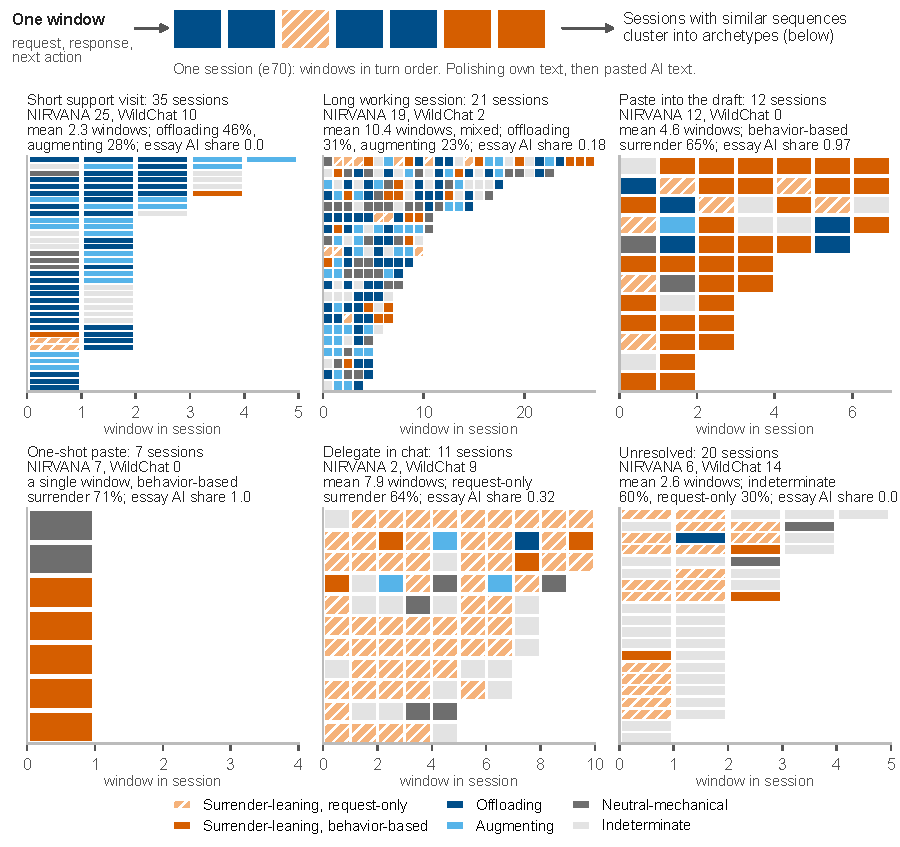
\includegraphics[width=\linewidth]{archetypes.pdf}
\caption{Top: a window is one tile, and a session is a row of windows in turn order. Below: every session, grouped into six archetypes by clustering category sequences. Percentages are mean shares of a session's windows. Essay AI share is the NIRVANA median of GPT Final \%, as a proportion; the Delegate in chat value rests on 2 NIRVANA sessions. Panels use different horizontal scales.}
\Description{Top strip: one window as a tile, then session e70 as seven tiles (offloading, offloading, request-only surrender, offloading, offloading, behavior-based surrender, behavior-based surrender). Below, six panels of rows of colored tiles. Short support visit, 35 sessions, and long working session, 21 sessions, are mostly offloading and augmenting. Paste into the draft, 12 sessions, and one-shot paste, 7 sessions, are mostly behavior-based surrender. Delegate in chat, 11 sessions, is mostly hatched request-only surrender. Unresolved, 20 sessions, is mostly indeterminate.}
\label{fig:archetypes}
\end{figure}
% src: analysis/results/mining.md s1, s8; analysis/results/mining/archetypes.csv

\begin{table}[tbp]
\caption{Use of AI by activity, and how the output was checked.}
\label{tab:aiuse}
\small
\begin{tabular}{p{0.17\linewidth}p{0.42\linewidth}p{0.31\linewidth}}
\toprule
Activity & What AI did & How output was checked \\
\midrule
Literature & Following the review structure I set, searched OpenAlex and arXiv by script, screened 713 records with Haiku 5.5 and Sonnet 5.5, read sources, drafted the related work and framework comparison & Fresh critic agents; registry records and identifiers; no human checked the screening \\
Study design & Turned my study design into a written plan, briefs, protocols and a rule table & I reviewed and accepted the plan; critic agents reviewed each stage \\
Dataset work & Built windows, labeled WildChat with Sonnet 5.5 (43 labels record Claude Sonnet 5 as served), audited the screen with Opus 5.5 & Scripted rebuilds and critic agents \\
Codebook & Drafted and revised v1.1 and v1.2 within the coding framework I built, using pilots by AI coders & I accepted v1.1 at a checkpoint; critic agents reviewed; no human coded with it \\
Coding & All coding: Opus 5.5 and Sonnet 5.5 coders, Opus 5.5 adjudicators, Fable 5.1 on the 20-window set & AI-to-AI agreement and transcript audits only \\
Analysis & Implemented my analysis framework in scripts, ran them, compiled results, and drafted figures and result summaries & Byte-identical reruns and skeptic agents \\
Writing & Used Opus 5.5 to draft the milestone report and paper around the narrative I set, connect sections, and revise wording & Spell-check script, a fresh proofreading agent and a fresh critic agent \\
Figures & Redrew the figures in one palette, replaced six tables with figures and added explanatory diagrams, using Opus 5.5 & Scripted rerun, palette and text-overlap checks, a fresh figure critic and its recheck; the recheck's minor corrections were applied afterward and not rechecked \\
Editing & Applied the proofreading and critic findings to the draft, using Opus 5.5 & A fresh critic rechecked the edits; its minor corrections were applied afterward and not rechecked \\
Disclosure & Codex revised the wording of the AI Use Statement & Compared the revision with the prior disclosure and project records \\
Condensing & Cut the body from 20 to 11 pages at my request and moved details, four figures and the full process record to a supplementary details file, using Opus 5.5 & A script checked each number against the longer draft; a fresh critic compared the two versions \\
\bottomrule
\end{tabular}
\end{table}

\end{document}
